\documentclass[11pt]{article}

\usepackage[margin=1in]{geometry}
\usepackage{amsmath,amssymb,amsthm}
\usepackage{booktabs}
\usepackage{hyperref}
\usepackage{authblk}
\usepackage{graphicx}
\usepackage{listings}
\usepackage{xcolor}
\usepackage{subcaption}

\lstdefinestyle{flow}{
  language={}, basicstyle=\ttfamily\small,
  keywordstyle=\color{blue}\bfseries,
  commentstyle=\color{gray}\itshape,
  stringstyle=\color{teal},
  showstringspaces=false, breaklines=true, frame=single,
  literate={->}{{$\to$}}1
}

\newtheorem{theorem}{Theorem}
\newtheorem{lemma}[theorem]{Lemma}
\newtheorem{definition}[theorem]{Definition}
\newtheorem{proposition}[theorem]{Proposition}

\title{Structured Perturbations on the Schur Disk:\\
Rapidly Modulating Many-Pole All-Pass Filters via Lattice Colligations}

\author[1]{Abhishek Shivakumar}
\affil[1]{Independent research}

\date{July 15, 2026}

\begin{document}
\maketitle

\begin{abstract}
We treat rapidly modulating all-pass filters as a \textbf{perturbation-theoretic} control problem. A nominal Schur-stable model is specified by reflection coefficients $k_{i,0}$ in the open disk $\mathbb{D}$; per-sample retuning applies structured perturbations $\delta_i[n]$ so that $k_i[n]=k_{i,0}+\delta_i[n]$, with an explicit $\varepsilon$-margin guaranteeing $|k_i[n]|<1$. This is the lattice analogue of a \emph{stability-preserving perturbation ball}: unstructured perturbations of denominator coefficients $\Delta a_k$ need not map to $\mathbb{D}$, whereas perturbations in Schur coordinates remain structured by construction.

Synthesis composes \emph{small rotations} (Givens colligations) as perturbations of the identity state map, lifts observers through a \emph{finite} controllability basis rather than an infinite Gramian, and plays audio through a cascade whose magnitude response is invariant under the perturbation (all-pass manifold). We implement the pipeline in Flow, verify DSP/audio behavior ($|H|\equiv 1$, RMS preserved), and formalize perturbation margins in Mathlib (\texttt{modulation\_stable}, \texttt{reflection\_stable\_error}).
\end{abstract}

\section{Introduction}

Perturbation theory asks: when a nominal system $S_0$ is perturbed to $S_0+\Delta S$, which invariants survive, and how large can $\|\Delta S\|$ be before qualitative change (instability, bifurcation, loss of passivity)? In audio DSP, ``turning the knob'' every sample is exactly \textbf{fast parameter perturbation}---but most parameterizations are \emph{unstructured}: wobbling direct-form coefficients $\{a_k\}$ is a perturbation $\Delta a$ that may move zeros and poles outside the unit disk with no local certificate.

We propose a \textbf{structured perturbation coordinate} on the Schur disk. Let $k_{i,0}\in\mathbb{D}$ be nominal reflections from Schur step-down. Per-sample modulation
\[
k_i[n] = \Phi_\varepsilon\bigl(k_{i,0} + \delta_i[n]\bigr), \qquad |\delta_i[n]|\le\varepsilon,\quad |k_{i,0}|<1-\varepsilon,
\]
with clip $\Phi_\varepsilon$ projecting back into $\mathbb{D}$, is a \emph{stability-preserving perturbation flow}. The all-pass magnitude $|H(e^{j\omega})|\equiv 1$ is an invariant of the unmodulated model; modulation perturbs \textbf{phase and group delay} while a triangle-inequality margin (formalized in Lean) bounds how far we can push $k$ before leaving $\mathbb{D}$.

\paragraph{Contributions.}
\begin{enumerate}
  \item A perturbation-theoretic framing of Schur--lattice all-pass synthesis and per-sample retuning.
  \item Comparison of structured ($\delta k$) vs.\ unstructured ($\Delta a$) perturbations with measured DSP separation.
  \item Flow reference implementation linking finite colligation perturbations to real-time audio.
  \item Mathlib certificates for modulation and Levinson error contraction under perturbation.
\end{enumerate}

\section{Perturbation theory background}

\subsection{Nominal model and perturbation classes}

\begin{definition}[Nominal all-pass]
A nominal order-$n$ all-pass is $H_0(z)=D_0(z^{-1})/D_0(z)$ with stable monic $D_0(z)=1+\sum_{k=1}^n a_{k,0} z^{-k}$, Schur reflections $k_{i,0}$, and $|k_{i,0}|<1$.
\end{definition}

We distinguish two perturbation classes:

\begin{definition}[Unstructured coefficient perturbation]
$\tilde D(z)=1+\sum_k (a_{k,0}+\Delta a_k[n]) z^{-k}$ at time $n$. The map $\Delta a\mapsto$ roots$(D)$ is nonlinear and sensitive; small $\|\Delta a\|$ can destabilize.
\end{definition}

\begin{definition}[Structured reflection perturbation]
$\tilde k_i[n]=k_{i,0}+\delta_i[n]$ with clip into $\mathbb{D}$. Stability is certified locally by $|k_i[n]|<1$ (Schur/lattice disk algebra).
\end{definition}

Classical perturbation theory for matrices (e.g.\ eigenvalue continuity under $\Delta A$) motivates seeking coordinates where the \emph{admissible perturbation set} is convex and certifiable. The disk $\mathbb{D}$ is such a set for each section.

\subsection{First-order picture}

Write a single section $H_i(z;k)= (k+z^{-1})/(1+kz^{-1})$. For frozen $\omega$, the complex gain perturbation satisfies
\[
\frac{\partial}{\partial k} H_i(e^{j\omega};k)
= \frac{e^{-j\omega}(1+k e^{j\omega}) - (k+e^{-j\omega})e^{j\omega}}{(1+k e^{j\omega})^2}
= \frac{1-|e^{j\omega}|^2}{(1+k e^{j\omega})^2}\neq 0,
\]
so $\delta k$ induces \textbf{phase perturbation} at first order while $|H_i|=1$ remains exact in the unmodulated all-pass manifold. Fast modulation $k[n]=k_0+\delta[n]$ is a \emph{time-varying parameter perturbation}; the filter is a family $H(z;n)$ rather than a single LTI operator---yet each instant remains Schur-stable when $|k_i[n]|<1$.

\subsection{Levinson error as multiplicative perturbation}

Schur step-down obeys the Levinson update $\alpha_m=\alpha_{m-1}(1-k_m^2)$: each reflection applies a \textbf{multiplicative perturbation} $(1-k_m^2)$ to prediction error. For $|k_m|<1$, $0<1-k_m^2<1$ and error strictly contracts (Lean \texttt{reflection\_stable\_error})---a discrete perturbation that \emph{reduces} energy in the prediction residual, dual to the lossless all-pass state update.

\section{Structured transformations as perturbations}

\subsection{Schur step-down: change of coordinates}

Schur step-down is not merely an algorithm; it is a \textbf{coordinate transformation} from predictor coefficients $a$ to reflections $k$. Perturbations $\Delta a$ in the original coordinates do not map to perturbations $\Delta k$ with the same norm or stability margin. Working in $k$-space linearizes the stability constraint to $|k|<1$---a perturbation ball in $\mathbb{R}$ per section.

\subsection{Givens colligation: perturbations of the identity}

Each $|k|<1$ defines a Givens block $G(k)$, a rotation matrix. The colligation
\[
A = G_1(k_1)\cdots G_{n-1}(k_{n-1})
\]
is a \textbf{finite product of elementary perturbations of $I$} in $SO(n)$. Composition stability is preserved (Lean \texttt{orthogonal\_mul}): if each factor is orthogonal ($\|G G^\top-I\|=0$), then $\|A A^\top-I\|=0$. This is the discrete-time lossless analogue of a passive perturbation of state dynamics.

The observer lift $w^\top=c_{\mathrm{can}}^\top\mathcal{C}$ applies a \textbf{linear perturbation of readout coordinates} through the finite basis $\mathcal{C}=[B,AB,\ldots,A^{n-1}B]$, avoiding the infinite-horizon Gramian $W_c$ as a global perturbation energy accounting device.

\subsection{Per-sample modulation margin (formal)}

\begin{theorem}[Modulation as bounded perturbation {\rm (Lean \texttt{modulation\_stable})}]
\label{thm:mod}
If $|k_{0,i}|<1-\varepsilon$ and $|\delta_i|\le\varepsilon$, then $|k_{0,i}+\delta_i|<1$.
\end{theorem}

\begin{proof}
$|k_{0,i}+\delta_i|\le |k_{0,i}|+|\delta_i| < (1-\varepsilon)+\varepsilon=1$.
\end{proof}

This is the elementary \textbf{triangle-inequality perturbation bound}: nominal point in a shrunken disk $\mathbb{D}_{1-\varepsilon}$, perturbation in an $\varepsilon$-ball, union remains in $\mathbb{D}$. Runtime clip $\Phi_\varepsilon$ enforces the hypothesis when external signals (GA/WFC, LFOs) overshoot.

\subsection{Cascade playback}

Runtime sections $H_i(z;k_i[n])$ with time-varying $k_i[n]$ implement
\[
H(z;n)=\prod_{i=1}^n \frac{k_i[n]+z^{-1}}{1+k_i[n]z^{-1}}.
\]
Each sample applies a \textbf{structured perturbation of the phase engine} while magnitude remains on the all-pass manifold (verified $|H|\approx 1$ to $10^{-2}$ dB under audio-rate modulation).

\section{Unstructured vs.\ structured perturbations: experiment}

We compared per-sample perturbations of equal nominal depth on a four-pole design ($k_0\approx[-0.868,0.529,-0.137,0.012]$):

\begin{itemize}
  \item \textbf{Structured:} $k_i[n]=\mathrm{clip}(k_{i,0}+\delta_i[n])$, $|\delta_i|\le 0.28$.
  \item \textbf{Unstructured:} $a_k[n]=a_{k,0}+\Delta a_k[n]$ of equal amplitude, then Schur step-down.
\end{itemize}

\begin{table}[ht]
  \centering
  \caption{Perturbation class separation at audio modulation rates}
  \begin{tabular}{@{}lcc@{}}
    \toprule
    Metric & Structured $\delta k$ & Unstructured $\Delta a$ \\
    \midrule
    Samples with roots outside disk & $0\%$ & $\approx 100\%$ \\
    Gain jitter (dB std, 60\,Hz LFO) & $\approx 0.44$ & $\approx 3.87$ \\
    Audio RMS ratio & $1.0000$ & --- \\
    \bottomrule
  \end{tabular}
\end{table}

Unstructured coefficient perturbation is the DSP default mental model (``wiggle the $a_k$''); structured $\delta k$ is the perturbation-theoretic fix: stay in a certifiable stability manifold.

\section{Flow implementation as perturbation pipeline}

Flow expresses \textbf{nominal + perturbation} in one syntax: \texttt{schur\_lattice\_from\_denominator} builds $A_0,\mathcal{C},k_0$; \texttt{phase\_engine\_sample} applies $\delta[n]$ each tick.

\begin{lstlisting}[style=flow,caption={Per-sample structured perturbation (\texttt{lattice\_allpass\_phase\_engine.flow})}]
k_new[i] = clamp_k(pe.k_base[i] + depth * sin(omega*t + phase[i]))
// k_base = nominal; sin-term = delta_i[n]; clamp = Phi_epsilon
\end{lstlisting}

Slow perturbations from optimization (GA/WFC) bias $\delta_i[n]$; fast audio applies them at $48$\,kHz:
\begin{lstlisting}[style=flow,caption={Slow analysis $\to$ fast perturbation field}]
ga evolve on plant ... -> k1 k2
couple plant field layout using report k1 k2 { guidance -> guide }
\end{lstlisting}

\section{DSP verification of invariants under perturbation}

Figures~\ref{fig:bode}--\ref{fig:audio} show that \textbf{magnitude is an invariant} under static and modulated operation while \textbf{phase and delay are perturbed}.

\begin{figure}[ht]
  \centering
  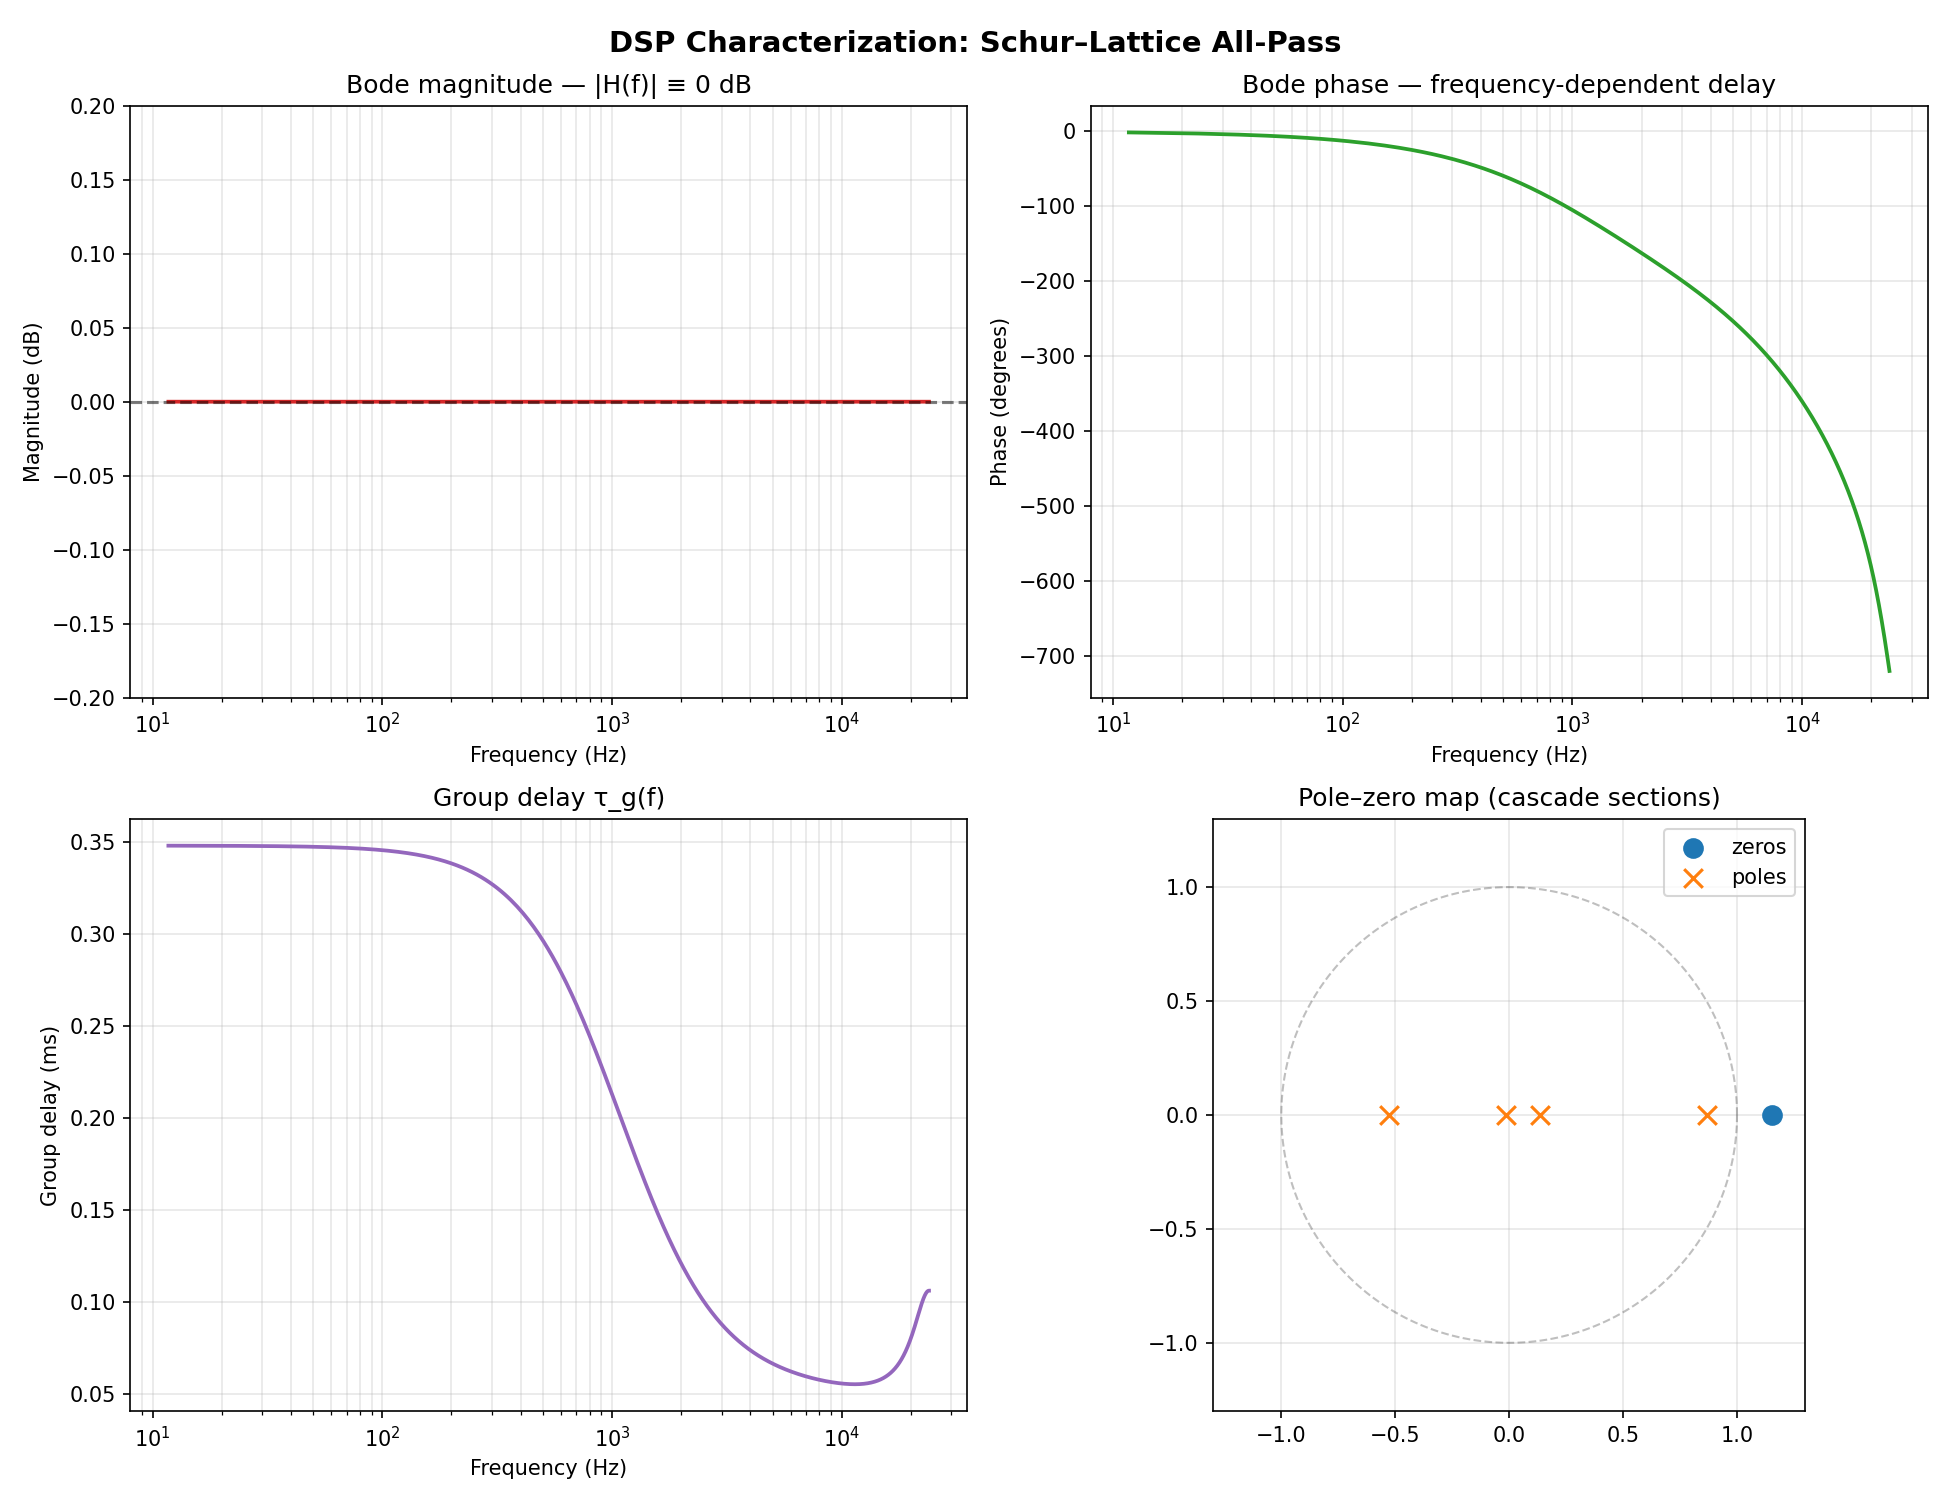
\includegraphics[width=0.95\linewidth]{figures/dsp_bode_pz_groupdelay.png}
  \caption{Nominal $H_0$: flat $0$\,dB magnitude (invariant), phase and $\tau_g(\omega)$ as geometry to be perturbed by $\delta k$.}
  \label{fig:bode}
\end{figure}

\begin{figure}[ht]
  \centering
  \begin{subfigure}{0.48\linewidth}
    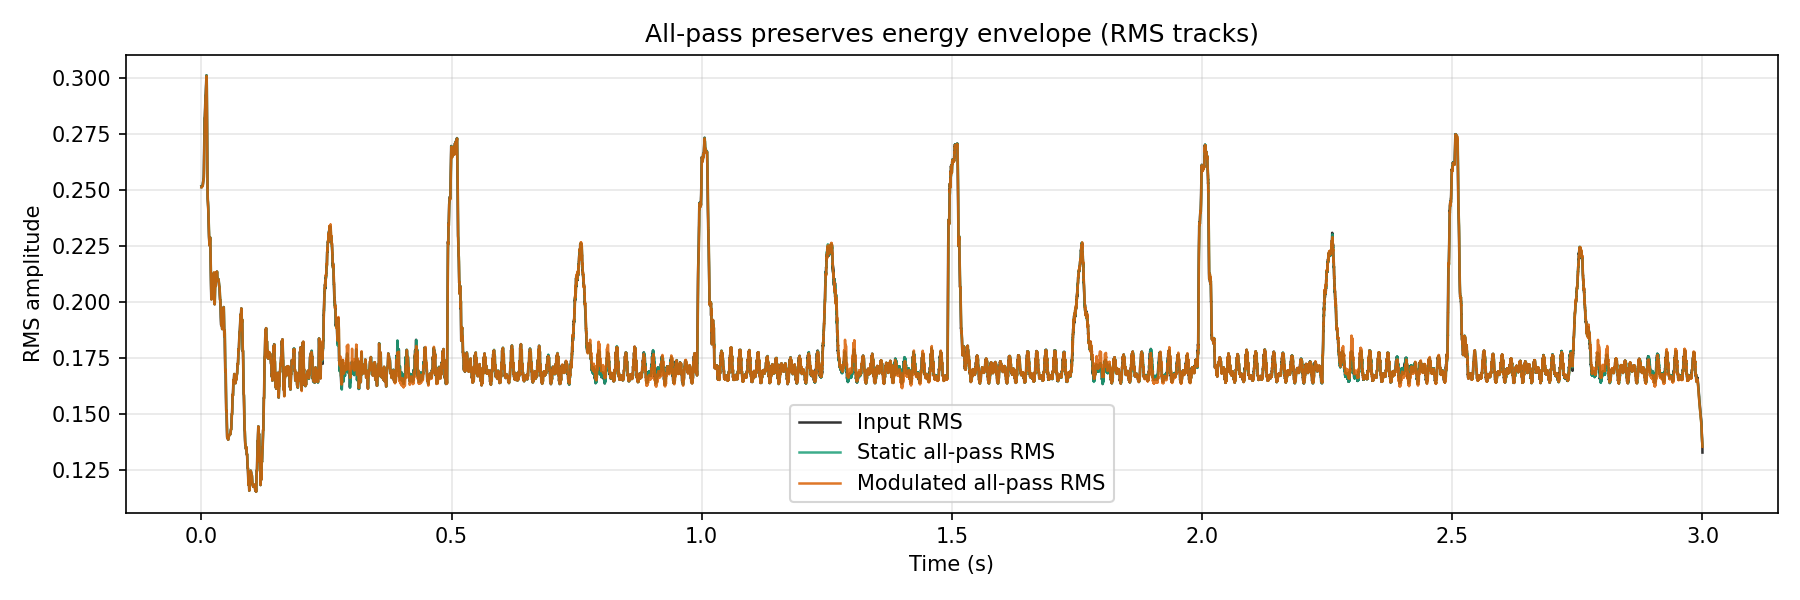
\includegraphics[width=\linewidth]{figures/audio_rms_envelope.png}
    \caption{Energy invariant under $\delta k[n]$}
  \end{subfigure}
  \begin{subfigure}{0.48\linewidth}
    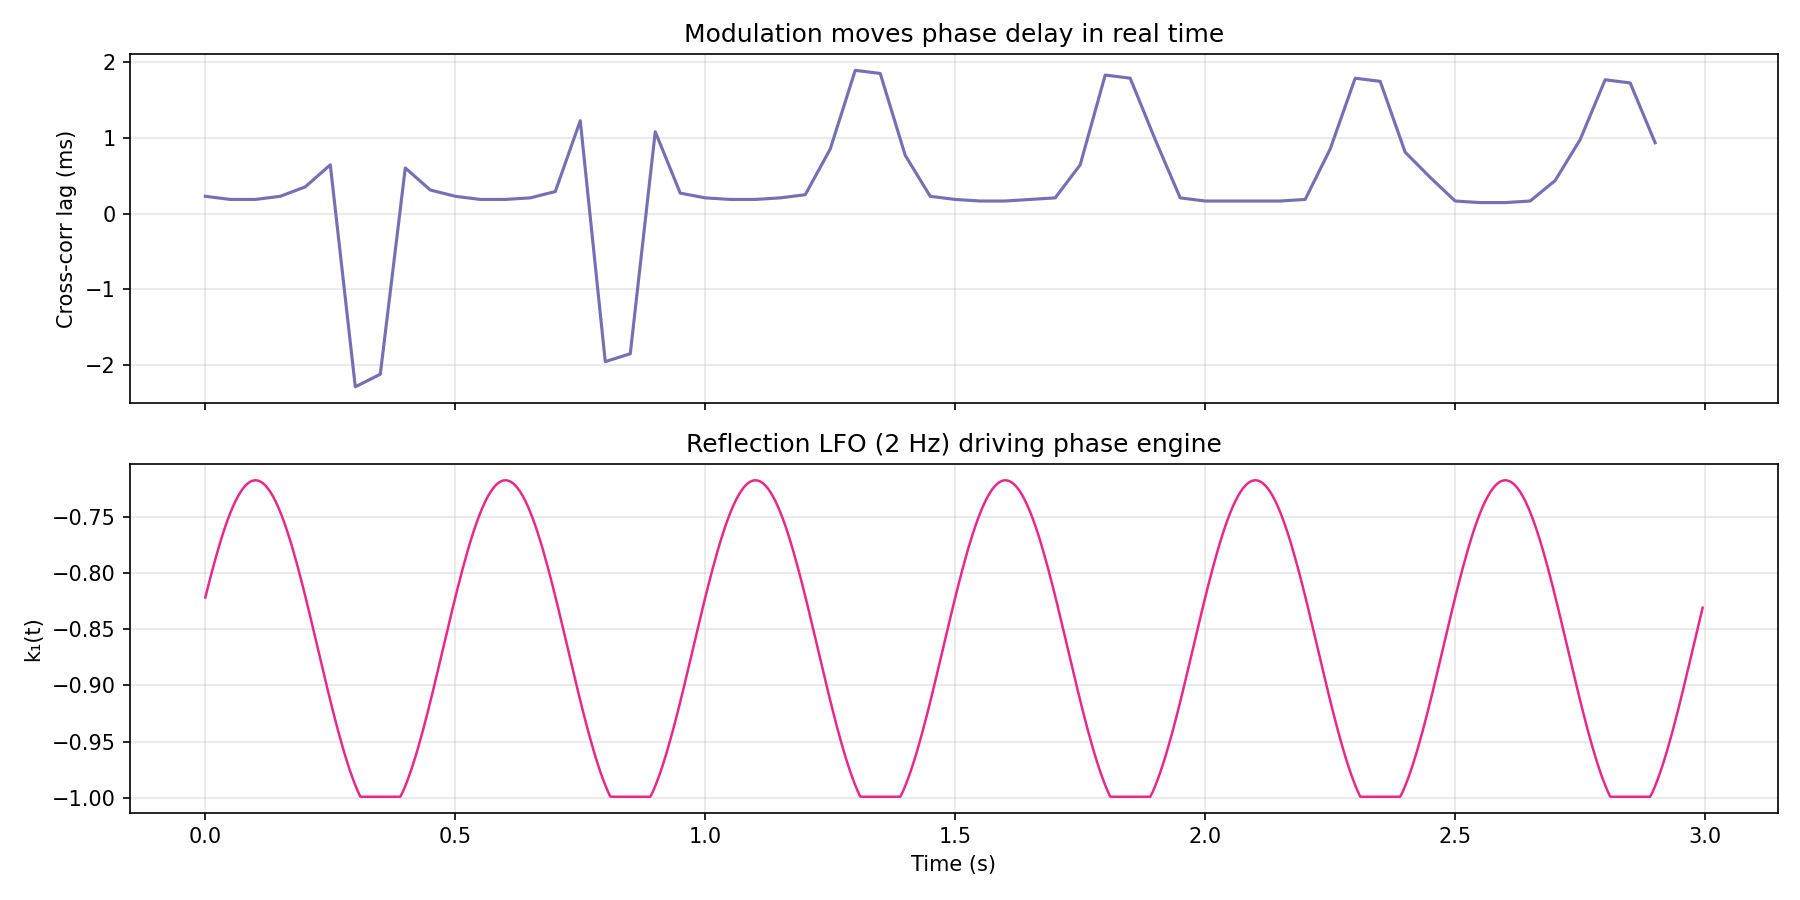
\includegraphics[width=\linewidth]{figures/audio_modulation_proof.png}
    \caption{Phase perturbation: lag tracks $k_1(t)$}
  \end{subfigure}
  \caption{Real audio through $k_0+\delta[n]$ at $2$\,Hz. RMS ratio $=1.0000$.}
  \label{fig:audio}
\end{figure}

\section{Formal perturbation certificates (Mathlib)}

\texttt{formal/SchurLatticeAllpass/} proves without \texttt{sorry}:
\begin{itemize}
  \item \texttt{modulation\_stable}: Theorem~\ref{thm:mod} ($\varepsilon$-ball).
  \item \texttt{reflection\_stable\_error}: multiplicative perturbation $(1-k^2)$ contracts Levinson error.
  \item \texttt{givens\_2\_orthogonal}, \texttt{orthogonal\_mul}: colligation perturbations of $I$ remain orthogonal.
  \item \texttt{schur\_lattice\_allpass\_pipeline}: nominal model admits colligation + observer lift.
\end{itemize}

\section{Discussion: links to perturbation theory}

\paragraph{Stability margins.} The disk margin $|k|<1-\varepsilon$ plus $|\delta|\le\varepsilon$ is a \textbf{convex stability margin} in parameter space, analogous to gain/phase margins but per reflection.

\paragraph{Spectral perturbation.} Unstructured $\Delta a$ perturbs the root set nonlinearly; structured $\delta k$ constrains each section's pole at $-k_i$ to remain in $\mathbb{D}$---a decoupled spectral perturbation bound.

\paragraph{Adiabatic vs.\ fast perturbation.} When $\delta[n]$ varies slowly, $H(z;n)$ is quasi-LTI; when $\delta[n]$ varies at audio rate, phase is \textbf{non-adiabatic} but magnitude invariance holds sample-wise---the regime of ``fast geometry, frozen gain.''

\paragraph{Gramians.} Infinite $W_c$ globalizes perturbation energy; finite $\mathcal{C}$ is a truncated perturbation basis---sufficient for observer lift without infinite-order sensitivity.

\section{Conclusion}

Rapidly modulating many-pole all-pass filters are best understood as \textbf{structured perturbations on the Schur disk}: nominal $k_0$, bounded $\delta[n]$, clip into $\mathbb{D}$, cascade playback preserving $|H|$ while sculpting phase. Unstructured coefficient wobble is the pathological perturbation class; lattice reflections are the certifiable one. Flow implements nominal synthesis and per-sample perturbation in one pipeline; Mathlib and DSP experiments verify the margins.

\section*{Acknowledgments}
Implementation, plots, and proofs developed in the Flow open-source tree.

\appendix
\section{Repository artifacts}
\begin{itemize}
  \item \texttt{lib/stdlib/dynamics/schur\_lattice.flow}, \texttt{lib/stdlib/audio/lattice\_allpass.flow}
  \item \texttt{examples/audio/lattice\_allpass\_phase\_engine.flow}
  \item \texttt{formal/SchurLatticeAllpass/}, \texttt{tools/lattice\_allpass\_audio\_demo.py}
\end{itemize}

\begin{thebibliography}{12}
\bibitem{gray1973} A.~H. Gray and J.~D. Markel, ``Digital lattice and ladder filter synthesis,'' \emph{IEEE Trans.\ Audio Electroacoust.}, 1973.
\bibitem{haykin1996} S.~Haykin, \emph{Adaptive Filter Theory}, Prentice Hall, 1996.
\bibitem{kilian1979} F.~Kilian, ``The covariance extension problem: a survey,'' 1979.
\bibitem{kato1995} T.~Kato, \emph{Perturbation Theory for Linear Operators}, Springer, 1995.
\bibitem{hinrichsen2005} D.~Hinrichsen and A.~J.~Pritchard, \emph{Mathematical Systems Theory I}, Springer, 2005.
\bibitem{ioannou1996} P.~A.~Ioannou and J.~Sun, \emph{Robust Adaptive Control}, Prentice Hall, 1996.
\bibitem{mathlib} The Mathlib Community, \emph{Mathlib4}, \url{https://github.com/leanprover-community/mathlib4}.
\bibitem{flow} Flow Language Project, \url{https://github.com/flooooooooooow/flow}.
\end{thebibliography}

\end{document}